% DSB overall architecture: BEVFusion (det + BEV seg) and FlashOCC (occ).
% Compile: pdflatex dsb_overview.tex  (or tectonic -X compile dsb_overview.tex)
\documentclass[tikz,border=8pt]{standalone}
% Shared styles for the DSB architecture diagrams.
\usepackage[T1]{fontenc}
\usepackage{graphicx}
\usetikzlibrary{arrows.meta, backgrounds, calc, fit, positioning, shapes.geometric}

\definecolor{camA}{HTML}{2A78D6}
\definecolor{lidA}{HTML}{1BAF7A}
\definecolor{fusA}{HTML}{EB6834}
\definecolor{detA}{HTML}{6250D6}
\definecolor{segA}{HTML}{0E8FA8}
\definecolor{occA}{HTML}{B5482A}
\definecolor{inkA}{HTML}{262626}
\definecolor{mutA}{HTML}{6B6B6B}

\tikzset{
  blk/.style={
    draw=inkA!70, line width=0.45pt, rounded corners=2.5pt,
    align=center, font=\small, inner sep=3pt,
    minimum height=0.95cm, text=inkA, fill=white,
  },
  cam/.style={blk, fill=camA!10, draw=camA!75},
  lid/.style={blk, fill=lidA!10, draw=lidA!75},
  fus/.style={blk, fill=fusA!12, draw=fusA!80},
  det/.style={blk, fill=detA!10, draw=detA!75},
  seg/.style={blk, fill=segA!10, draw=segA!75},
  occ/.style={blk, fill=occA!10, draw=occA!75},
  io/.style={blk, fill=black!4, draw=inkA!55},
  arr/.style={-{Stealth[length=2.2mm,width=1.6mm]}, line width=0.65pt, draw=inkA!75},
  darr/.style={arr, dashed},
  tag/.style={font=\scriptsize, text=mutA},
  grp/.style={draw=mutA!70, dashed, line width=0.6pt, rounded corners=6pt, inner sep=8pt},
  hdr/.style={font=\normalsize\bfseries, text=inkA, anchor=west},
  note/.style={font=\scriptsize, text=mutA, align=left},
}


\begin{document}
\begin{tikzpicture}

% ================================================================ shared inputs
\node[inner sep=1pt, draw=inkA!40, line width=0.5pt, rounded corners=2pt, fill=black] (lidar_in) at (0,17)
  {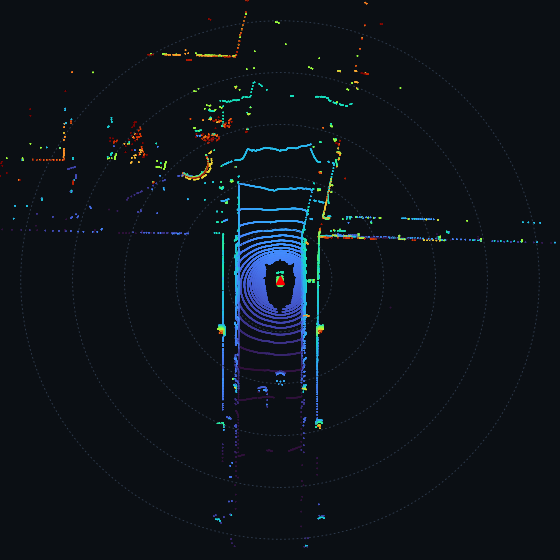
\includegraphics[width=2.5cm]{figs/lidar_bev.png}};
\node[tag, anchor=north] at (0,15.45) {LiDAR point cloud (BEV)};

\node[io, text width=3.6cm] (extr) at (0,9.0)
  {\textbf{Extrinsics / aug}\\camera2lidar $\cdot$ lidar2ego\\
   img\_aug $\cdot$ lidar\_aug};

\node[inner sep=1pt, draw=inkA!40, line width=0.5pt, rounded corners=2pt, fill=white] (cam_in) at (0,4.5)
  {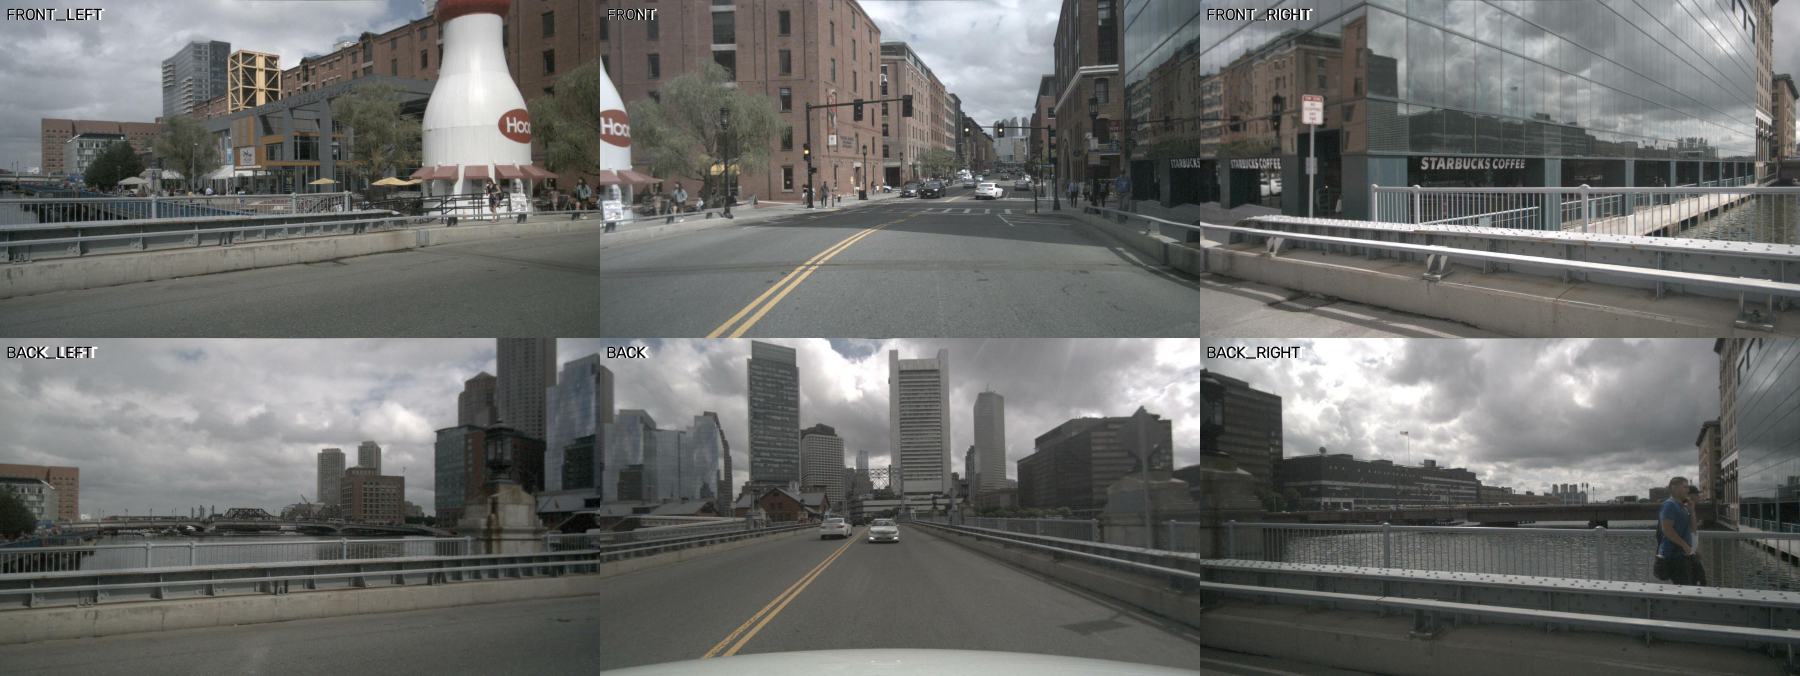
\includegraphics[width=4.0cm]{figs/cameras.png}};
\node[tag, anchor=north, text width=5.2cm] at (0,3.35)
  {6 cameras (shared by both networks)};

% ================================================================ BEVFusion: LiDAR row
\node[lid] (vox) at (4.6,17) {Voxelize\\0.075 m (xy) $\cdot$ 0.2 m (z)};
\node[lid] (scn) at (8.8,17) {SparseEncoder\\spconv};
\node[io]  (lid_bev) at (13.2,17) {LiDAR BEV\\256$\times$180$\times$180};

% ================================================================ BEVFusion: camera row
\node[cam] (swin) at (4.6,12.5) {Swin-T\\+ GeneralizedLSSFPN};
\node[cam] (vt)   at (8.8,12.5) {DepthLSS / LSS\\view transform};
\node[io]  (cam_bev) at (13.2,12.5) {camera BEV\\80$\times$180$\times$180};

% ================================================================ BEVFusion: fusion + heads
\node[fus] (fuser) at (17.6,14.75) {ConvFuser\\80+256 $\to$ 256};
\node[fus] (decoder) at (21.8,14.75) {SECOND + SECONDFPN\\512$\times$180$\times$180};
\node[det, text width=3.0cm] (object) at (26.2,17)   {\textbf{TransFusion} head\\3D detection};
\node[seg, text width=3.0cm] (map)    at (26.2,12.5) {\textbf{BEV seg} head\\6-class map};

% ================================================================ FlashOCC row
\node[cam] (r50)     at (4.6,4.5)  {ResNet-50\\+ CustomFPN};
\node[cam] (lss_occ) at (8.8,4.5)  {LSSViewTransformer\\64$\times$200$\times$200};
\node[cam] (bevenc)  at (13.4,4.5) {CustomResNet\\+ FPN\_LSS\\256$\times$200$\times$200};
\node[occ] (occhead) at (17.8,4.5) {BEVOCCHead2D\\$18\times16$ channels};

% ================================================================ input routing
\draw[arr] (lidar_in.east) -- (vox.west);
\draw[arr] (cam_in.east) -- (r50.west);
% camera: up one row into the BEVFusion camera branch
\draw[arr] (cam_in.east) -- (2.0,11.4) -- (4.6,11.4) -- (swin.south);
% extrinsics: vertical bus at x=2.6, taps to LSS (below) and vtransform (above)
\draw[darr] (extr.east) -- (2.6,9.0);
\draw[darr] (2.6,14.0) -- (2.6,6.4);
\node[tag, rotate=90] at (2.38,11.0) {geometry};
\draw[darr] (2.6,14.0) -- (8.8,14.0) -- (vt.north);
\draw[darr] (2.6,6.4)  -- (8.8,6.4)  -- (lss_occ.north);

% ================================================================ BEVFusion dataflow
\draw[arr] (vox) -- (scn);
\draw[arr] (scn) -- (lid_bev);
\draw[arr] (swin) -- (vt);
\draw[arr] (vt) -- (cam_bev);
\draw[arr] (lid_bev.east) -| (fuser.north);
\draw[arr] (cam_bev.east) -| (fuser.south);
\draw[arr] (fuser) -- (decoder);
\draw[arr] (decoder.east) -| (object.west);
\draw[arr] (decoder.east) -| (map.west);

% ================================================================ FlashOCC dataflow
\draw[arr] (r50) -- (lss_occ);
\draw[arr] (lss_occ) -- (bevenc);
\draw[arr] (bevenc) -- (occhead);

% ================================================================ outputs (real inference)
\node[inner sep=1.5pt, draw=inkA!40, line width=0.5pt, rounded corners=3pt, fill=white] (det_out) at (33,18)
  {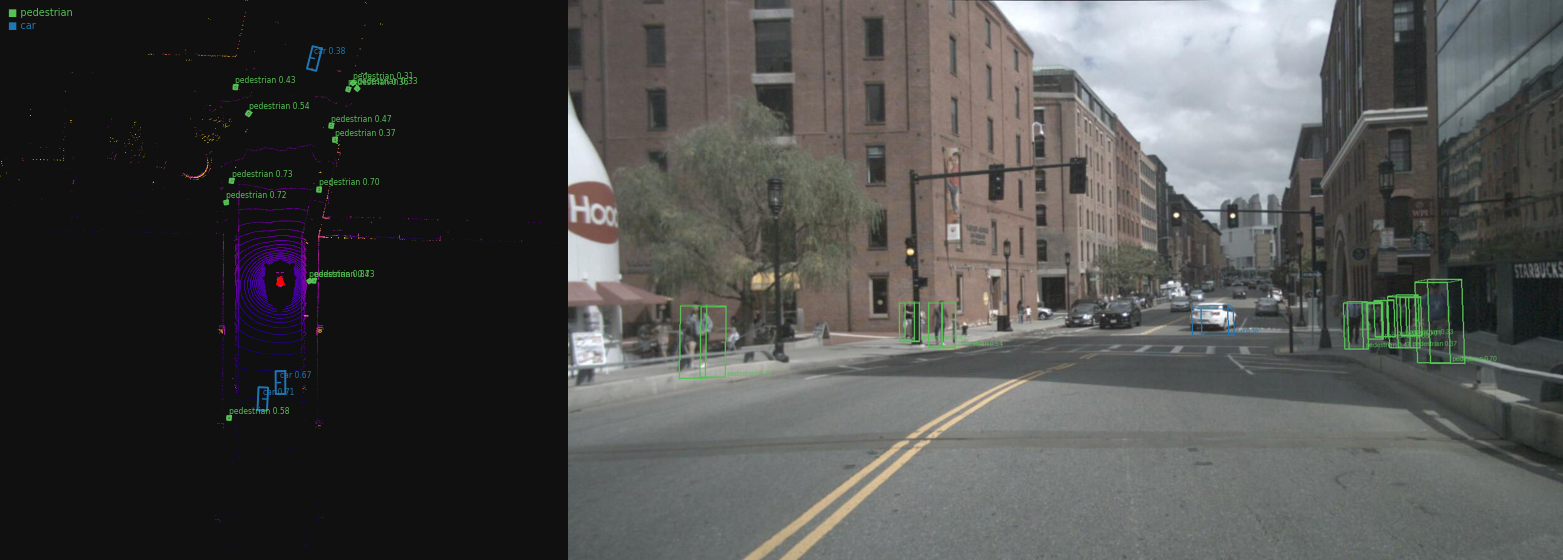
\includegraphics[width=5.6cm]{figs/det_result.png}};
\node[tag, anchor=north] at (33,15.6) {detection: 6 cameras + centered BEV};
\draw[arr] (object.east) -| (det_out.west);

\node[inner sep=1.5pt, draw=inkA!40, line width=0.5pt, rounded corners=3pt, fill=white] (seg_out) at (33,11.2)
  {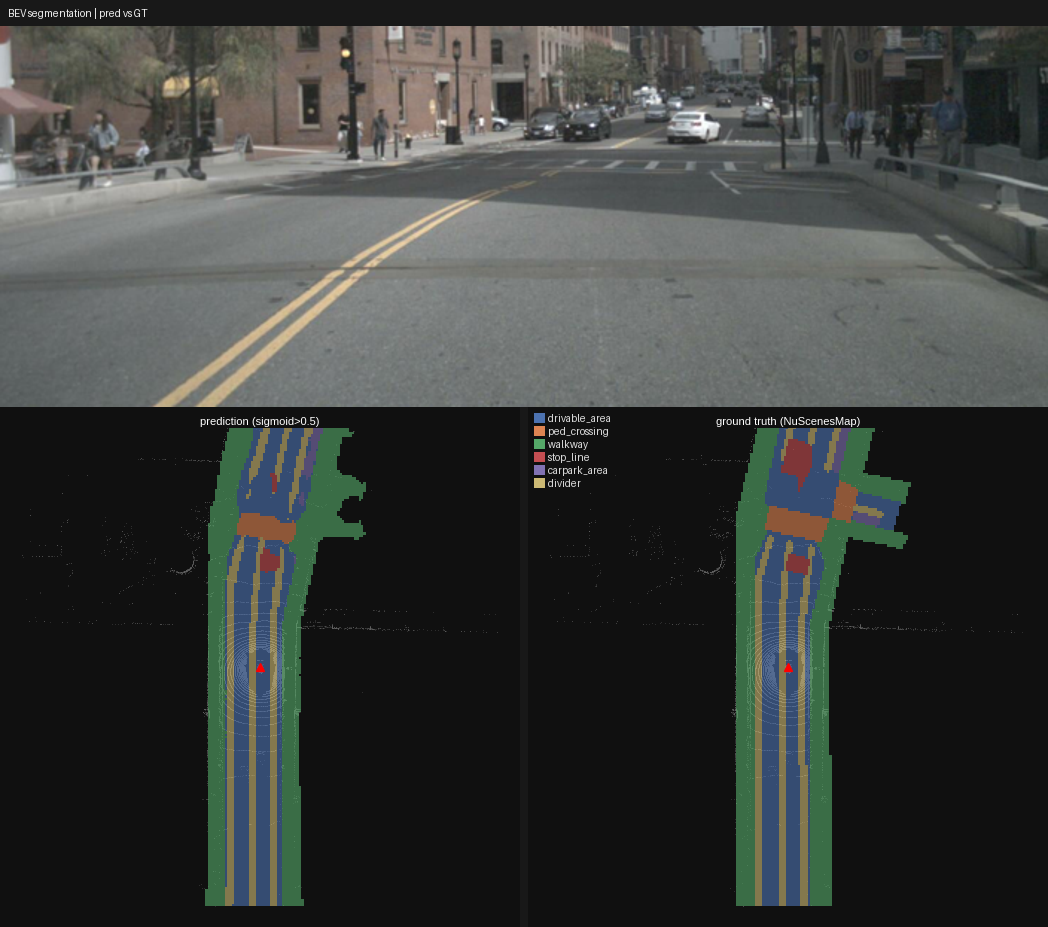
\includegraphics[width=4.0cm]{figs/seg_result.png}};
\node[tag, anchor=north] at (33,8.8) {BEV segmentation: pred vs GT};
\draw[arr] (map.east) -| (seg_out.west);

\node[inner sep=1.5pt, draw=inkA!40, line width=0.5pt, rounded corners=3pt, fill=white] (occ_out) at (33,4.0)
  {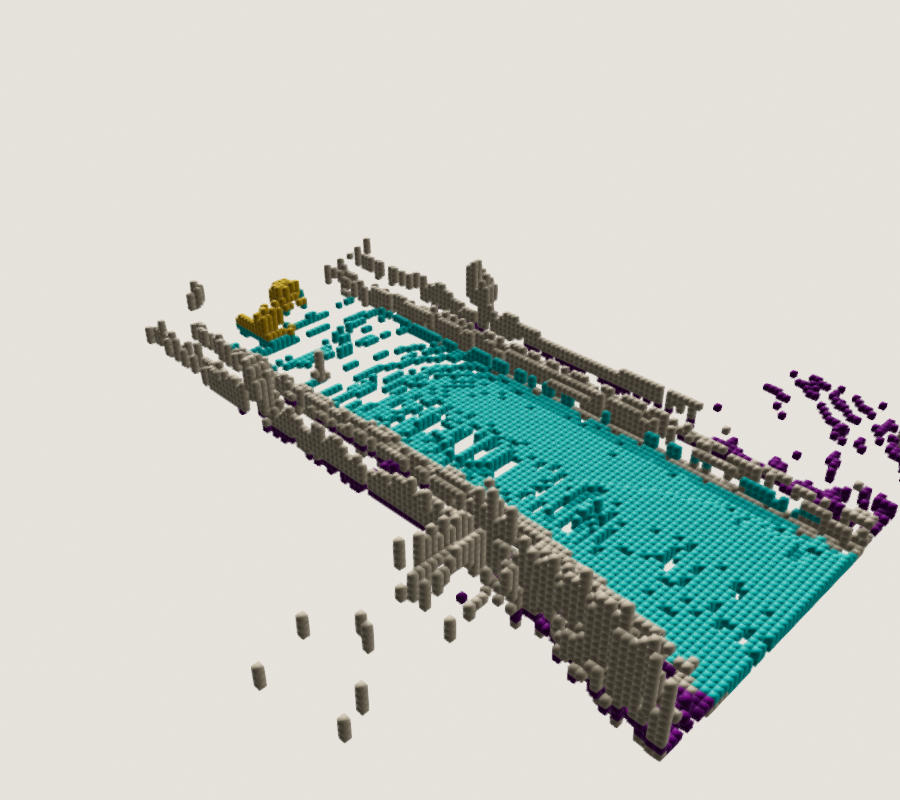
\includegraphics[width=3.3cm]{figs/occ_result.png}};
\node[tag, anchor=north] at (33,2.25) {occupancy: 200$\times$200$\times$16};
\draw[arr] (occhead.east) -| (occ_out.west);

% ================================================================ groups / titles
\begin{scope}[on background layer]
  \node[grp, fit=(vox)(scn)(lid_bev)(swin)(vt)(cam_bev)(fuser)(decoder)(object)(map),
        label={[tag]above:BEVFusion \textbar{} camera + LiDAR}] {};
  \node[grp, fit=(r50)(lss_occ)(bevenc)(occhead),
        label={[tag]below:FlashOCC \textbar{} camera only}] {};
\end{scope}

\node[hdr] at (2.8,21.2) {DSB perception: BEVFusion (detection + BEV segmentation) and FlashOCC (occupancy)};
\node[note, anchor=north west, text width=20cm] at (2.8,20.6)
  {BEVFusion: Swin-T + LSS/DepthLSS (camera) and SparseEncoder (LiDAR) $\to$ ConvFuser $\to$ TransFusion / BEV-seg heads.
   FlashOCC: ResNet-50 + LSS view transform + 2D BEV encoder + channel-to-height occupancy head.
   Both consume the same 6 cameras; the image backbones differ (Swin-T vs ResNet-50).};
\node[note, anchor=north west, text width=30cm] at (-1.6,-0.8)
  {Grids: det 0.075$\times$0.075$\times$0.2 m voxel / 180$\times$180 BEV; seg 0.1$\times$0.1$\times$0.2 m voxel / 128$\times$128 BEV
   (+ 200$\times$200 map @ 0.5 m); occ 0.4 m / 200$\times$200$\times$16 occupancy.};

\end{tikzpicture}
\end{document}
